\documentclass{article}
\usepackage[T1]{fontenc}
\usepackage{lmodern}
\usepackage{graphicx}
\usepackage{amsmath,amssymb}
\usepackage[a4paper,margin=2cm]{geometry}
\usepackage[absolute,overlay]{textpos}
\setlength{\TPHorizModule}{1mm}
\setlength{\TPVertModule}{1mm}
\usepackage[indonesian]{babel}
\usepackage{hyperref}
\setlength{\emergencystretch}{2em}
% unit: Halaman 15

\begin{document}

% === Halaman 15 (llm) ===

\begin{itemize}
  \item Pada mode ECB, blok plainteks yang sama selalu dienkripsi menjadi blok cipherteks yang sama.
\end{itemize}

\vspace{10mm}

\begin{itemize}
  \item Pada contoh di atas, blok 1010 muncul dua kali dan selalu dienkripsi menjadi 0010.
\end{itemize}

% deskripsi: Ilustrasi proses enkripsi mode ECB yang menunjukkan operasi XOR antara plainteks dan kunci, pergeseran bit, dan konversi ke notasi HEX, dengan penekanan pada blok 1010 yang menghasilkan output 0010 secara konsisten.
% bbox normalisasi: [0.1600, 0.2900, 0.7600, 0.6100]
\begin{textblock*}{126.00mm}(33.60mm,86.13mm)
\noindent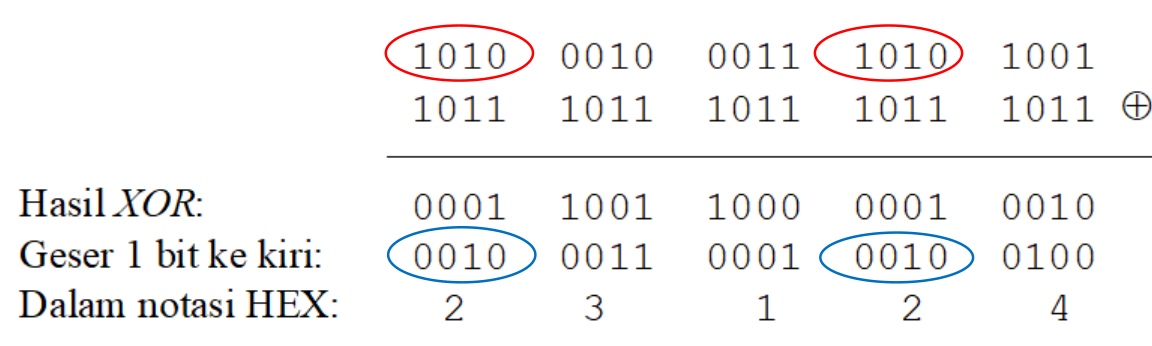
\includegraphics[width=126.00mm,height=95.04mm]{../../images/llm/page_015_img_01.png}%
\end{textblock*}

\end{document}
